
\documentclass[12pt]{article}
 
\usepackage[utf8]{inputenc}
\usepackage[T1]{fontenc}
\usepackage[german]{babel}
\usepackage{graphicx}
\usepackage{cleveref}
\usepackage{wrapfig}
\usepackage{amsmath}
\usepackage{amsfonts}
\usepackage{amssymb}
\usepackage{tikz}
\usepackage{nicefrac}
\usepackage{mathtools}
\usepackage[margin=1in]{geometry}
\usepackage[section]{placeins}

\newcommand{\kq}{\frac{1}{4 \pi \epsilon_0}}

\newenvironment{solution}{\begin{proof}[Solution]}{\end{proof}}
 
\begin{document}
 
\title{Experimental Physik III}
\author{Wichtiges\\ 
Andréz Gockel\\}
 
\date{\today}
\maketitle

\section{Relativitäts Theorie}

\subsection{Experimente}
\paragraph{Fizeau-Experiment}

In den beiden Rohren der Länge l fließt eine Flußigkeit mit dem Brechungsindex $n$ mit einer Geschwindigkeit $v$. Licht der Wellenlänge $\lambda$ wird durch einen Strahlteiler (BS) aufgeteilt, und die beiden Strahlen werden von den Spiegeln M2, M3, M4 so reflektiert, dass sie vor dem Auftreffen auf die Kamera die gleiche Strecke zuru ̈cklegen; der eine Strahl im Uhrzeigersinn (BS → M2 → M3 → M4 → BS) und der Andere gegen den Uhrzeigersinn (BS → M4 → M3 →M2 →BS).

\begin{figure}
\centering
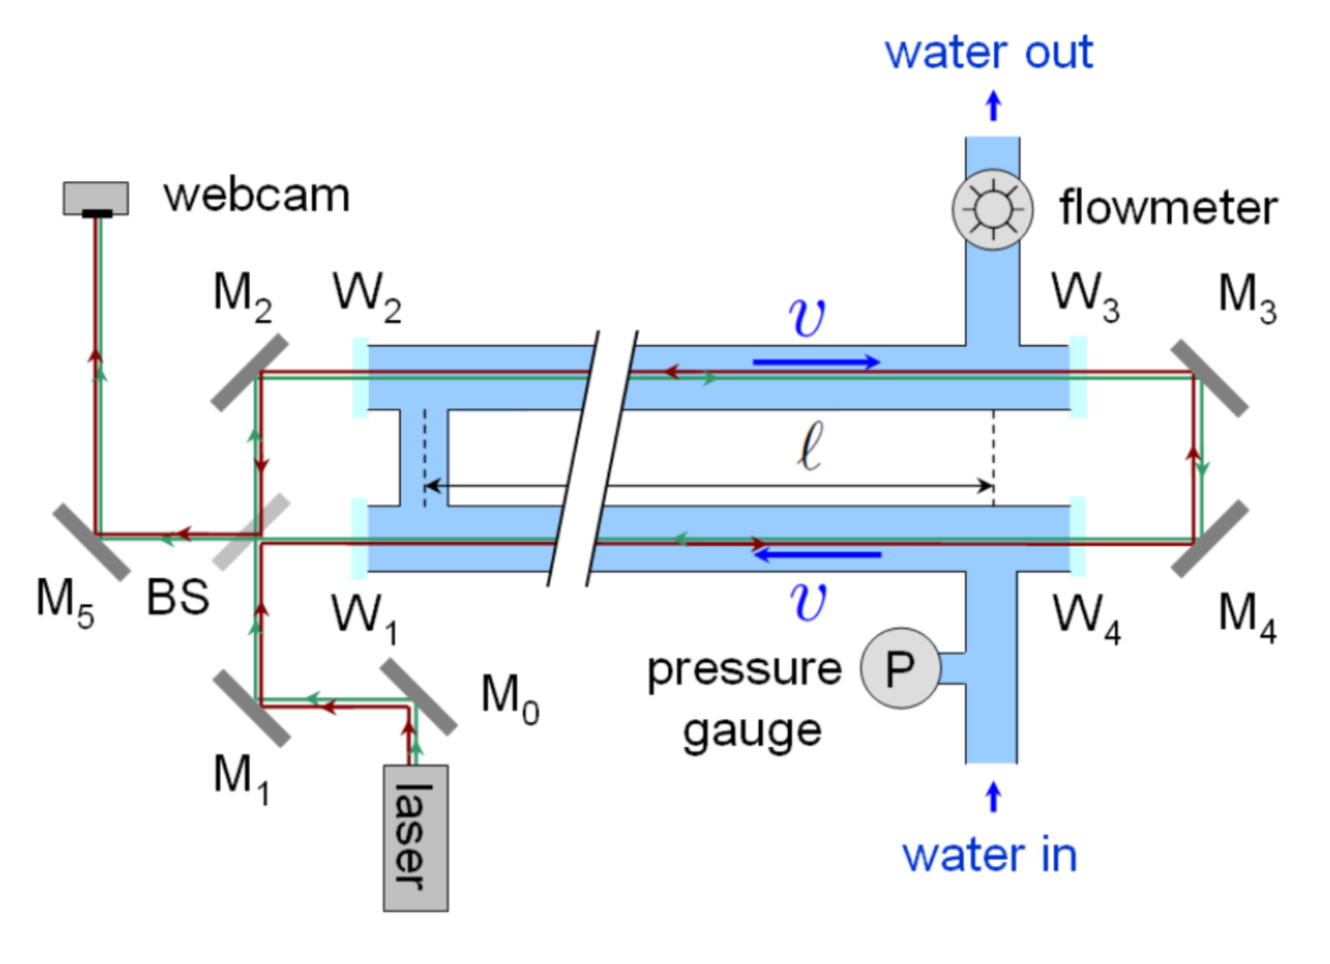
\includegraphics[width=.8\textwidth]{Fizz}
\caption{Fizeau-Experiment}
\label{fizz}
\end{figure}




\end{document}